\chapter{Classification of Spectra}
\label{ch:spectra_classification}

\begin{wrapfigure}{o}{0.82\textwidth}
    \centering
    \vspace{-3.4cm}
    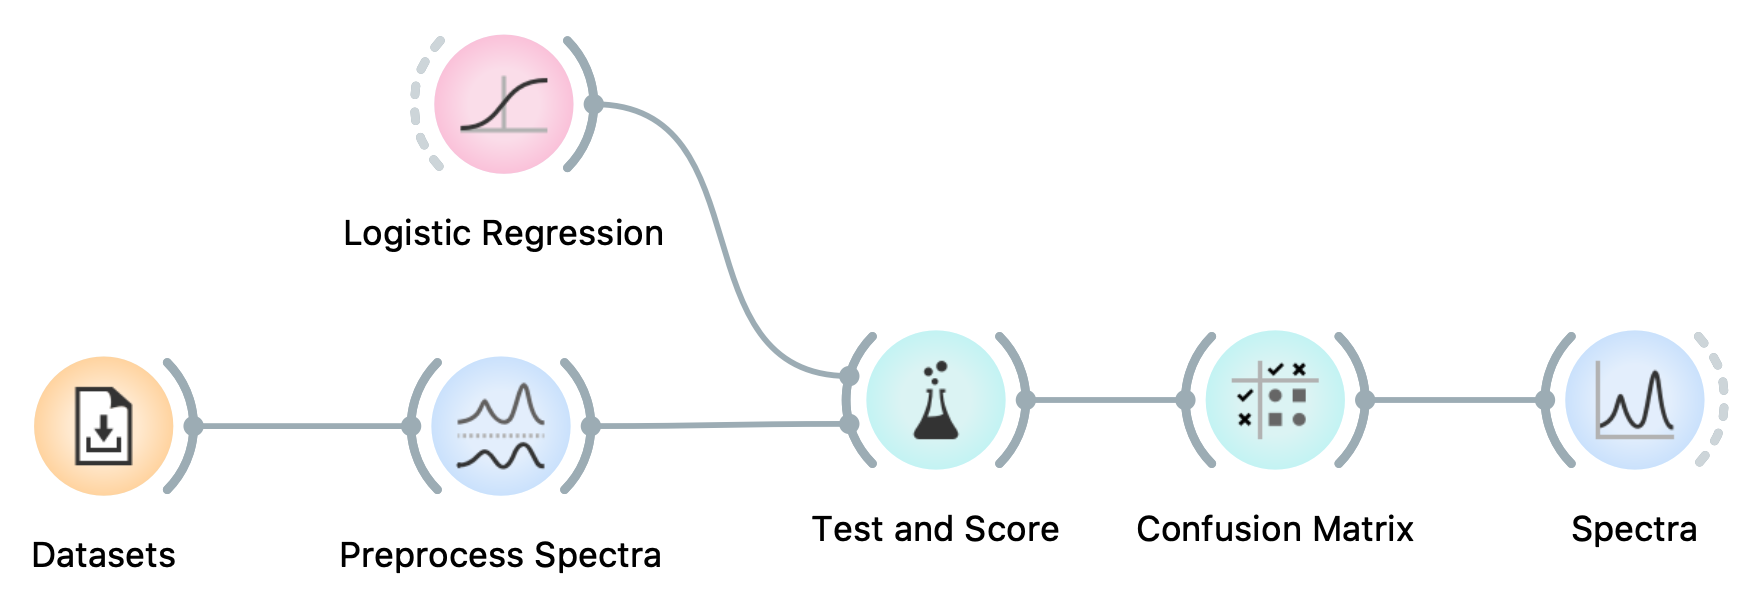
\includegraphics[width=0.95\textwidth]{graphics/ch-spectra_classification/sp_classification-fig1.png}
    \label{fig:spectra_classification-fig1}
\end{wrapfigure}


Let’s open the collagen data set again and see how well can logistic regression predict its four classes. Straightforward, right? Connect \widget{Datasets}, \widget{Logistic Regression}, \widget{Predictions}, \widget{Confusion Matrix} and that's it. We would also like to do some spectral processing (we will only keep the columns for wavenumbers between 1500\wn and 1800\wn).

\begin{figure}[h]
\hspace{-1cm}\stackinset{r}{-0.7\linewidth}{t}{+0.25\linewidth}
  {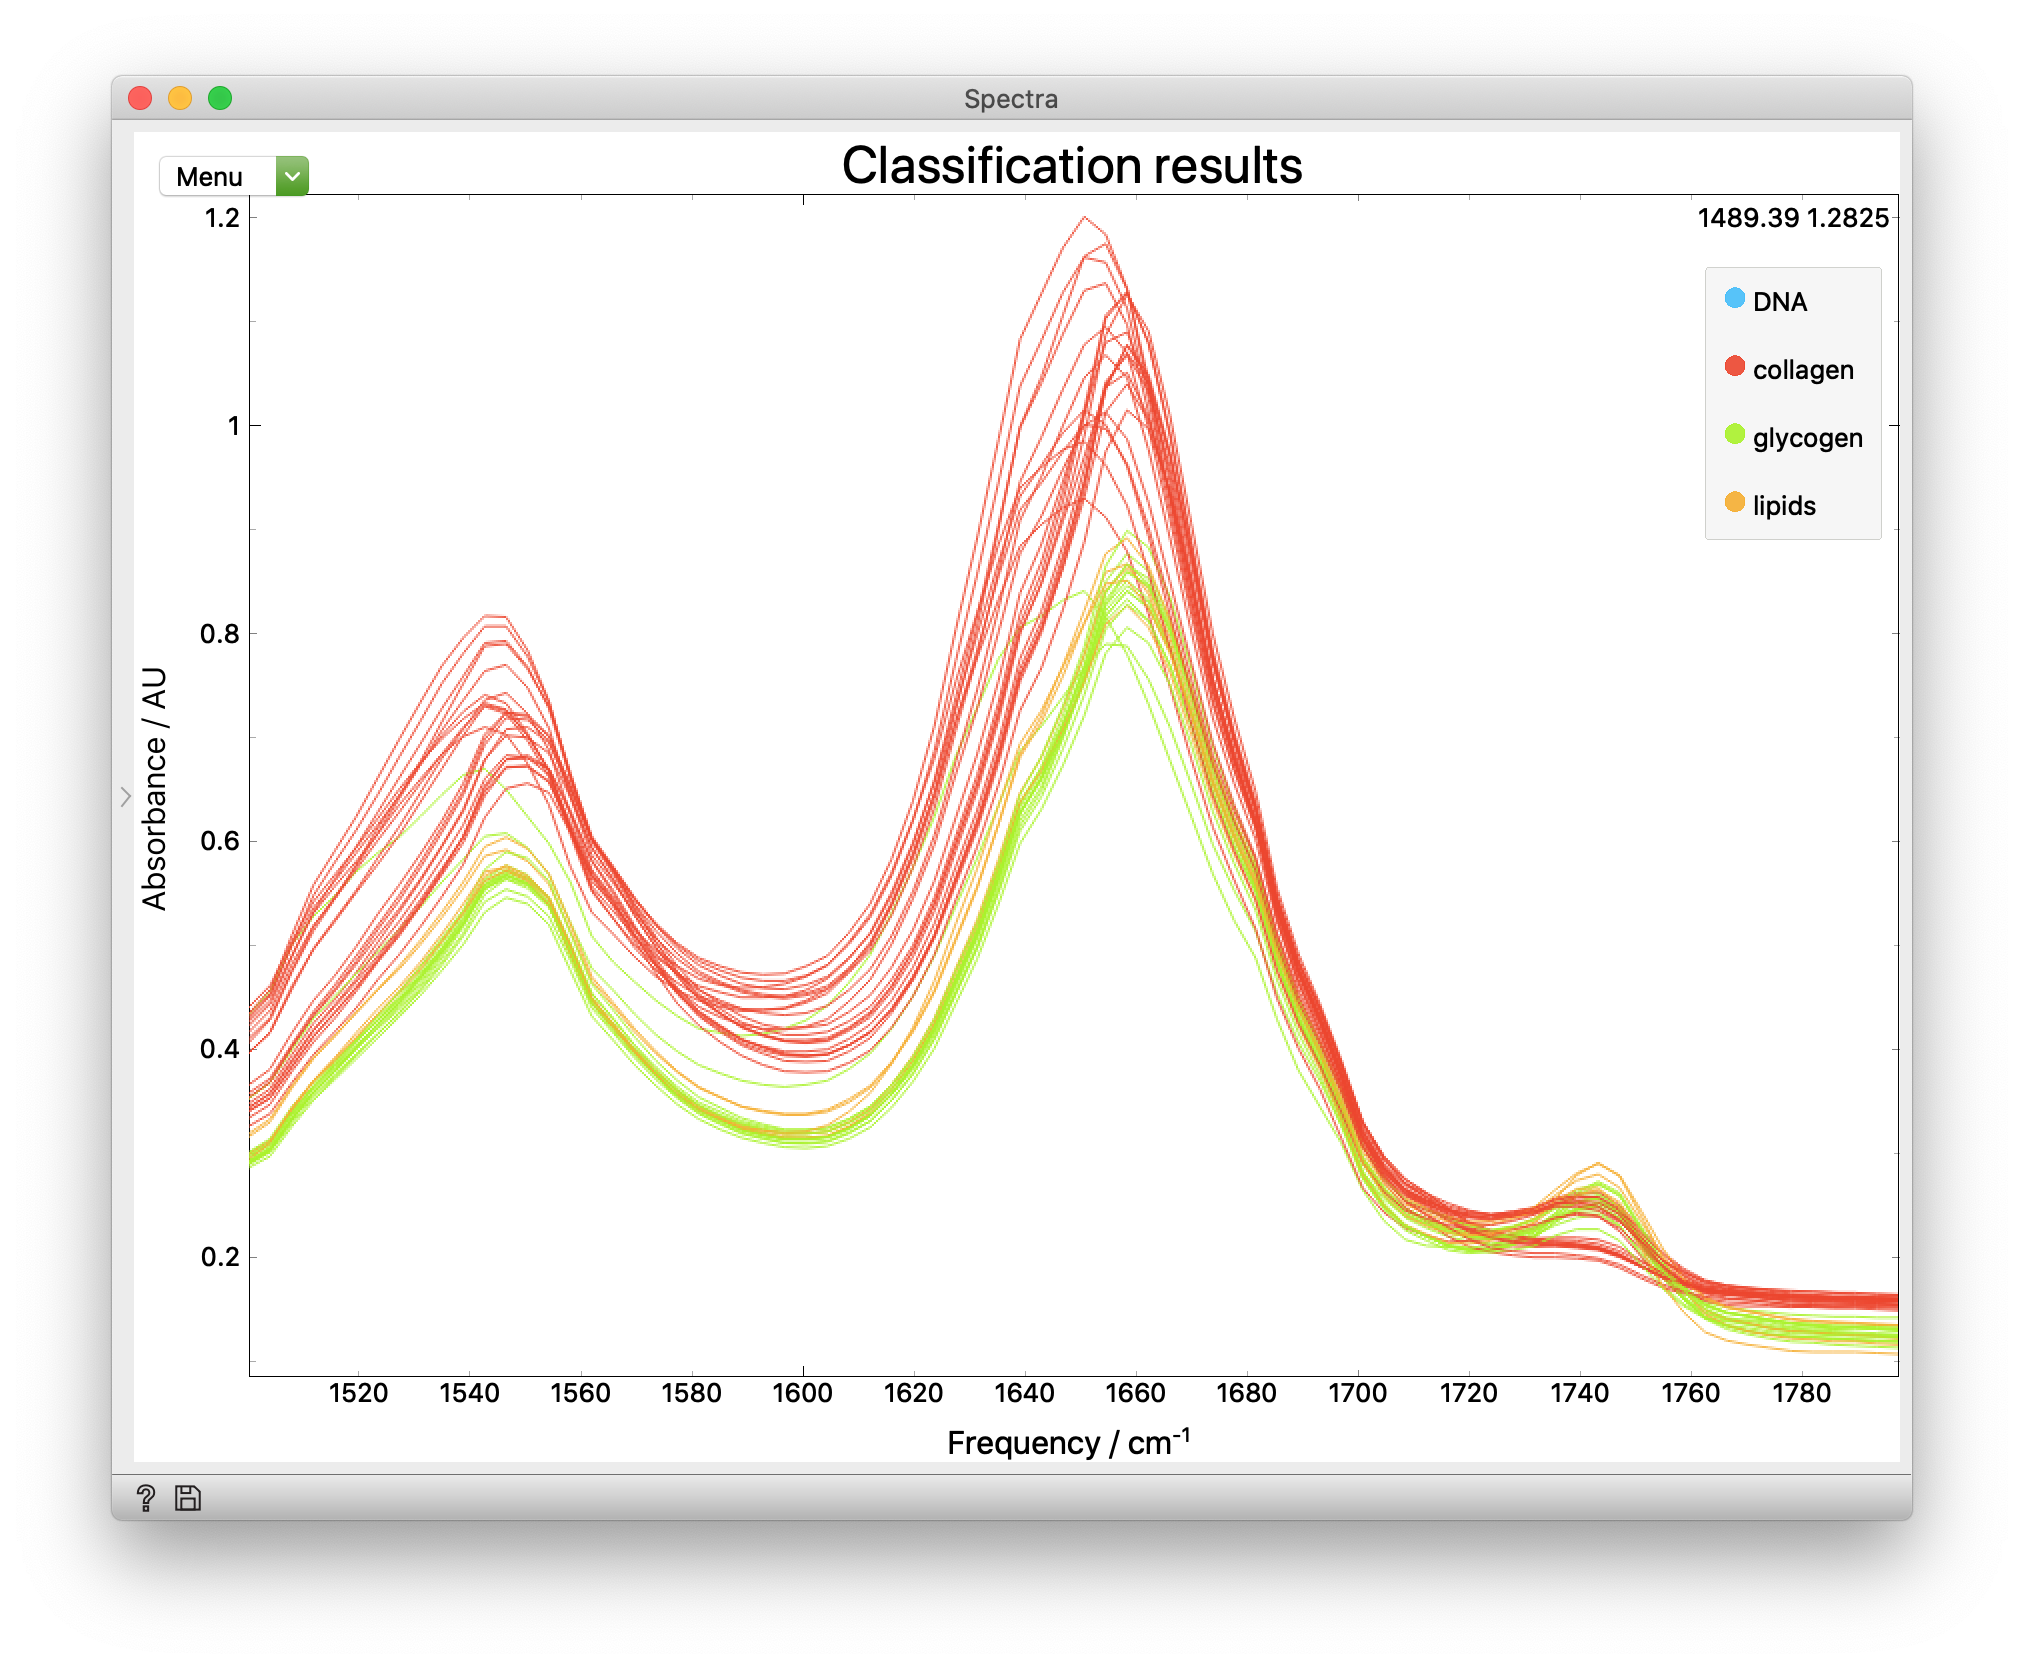
\includegraphics[scale=0.35]{graphics/ch-spectra_classification/sp_classification-fig2b.png}}
  {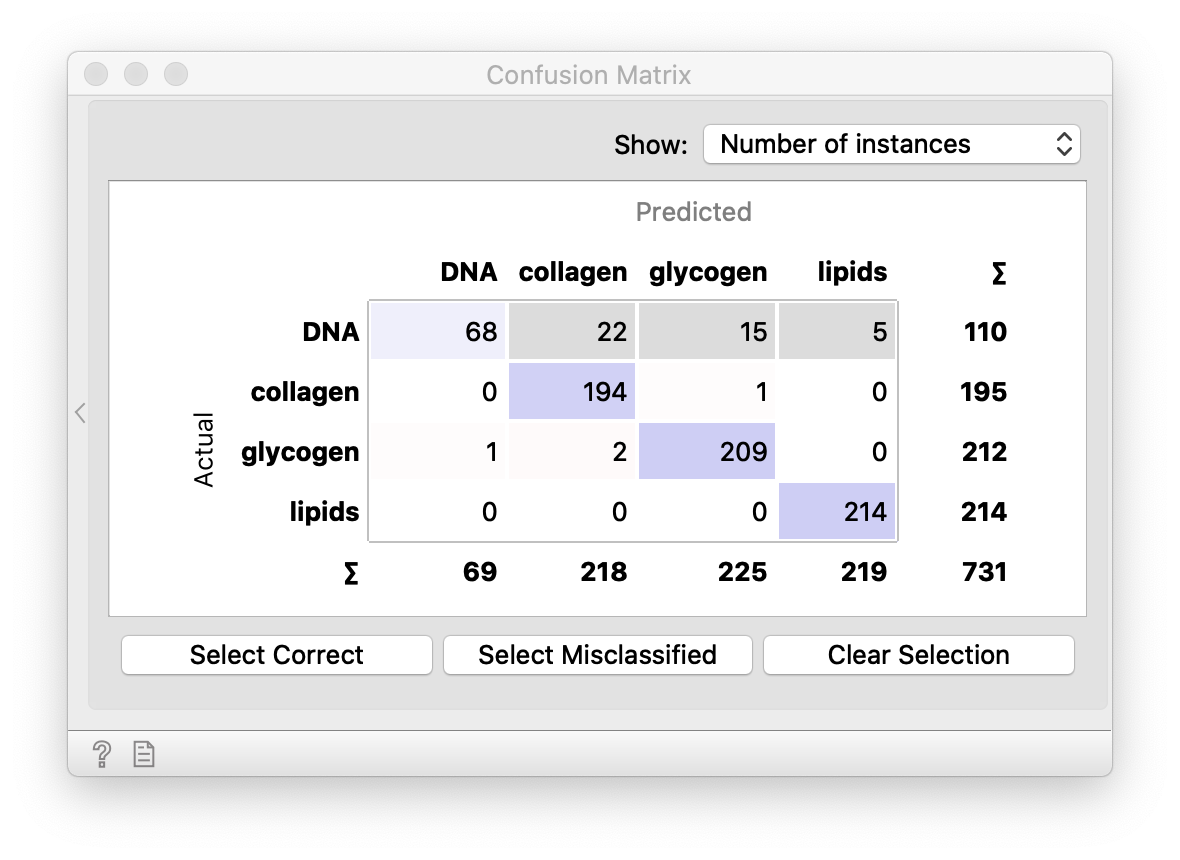
\includegraphics[scale=0.45]{graphics/ch-spectra_classification/sp_classification-fig2a_.png}}
  \caption{The \widget{Spectra} widget shows wrong predictions for the DNA class.}
  \label{ffig:spectra_classification-fig2}
\end{figure}

Let’s not forget that it is pointless to predict for the same data as we used for learning. We could either  use a \widget{Data Sampler} and connect its Sample output to \widget{Preprocess Spectra} and Remaining output to \widget{Predictions}, or obtain predictions from the \widget{Test and Score} widget.
\widget{Confusion Matrix} now shows the mistakes of the model (scored with cross-validation). We can select them and inspect them further in a \widget{Spectra} widget. Here we colored them by the predicted class (see the Menu). 

\begin{wrapfigure}{o}{1.1\textwidth}
  \centering
  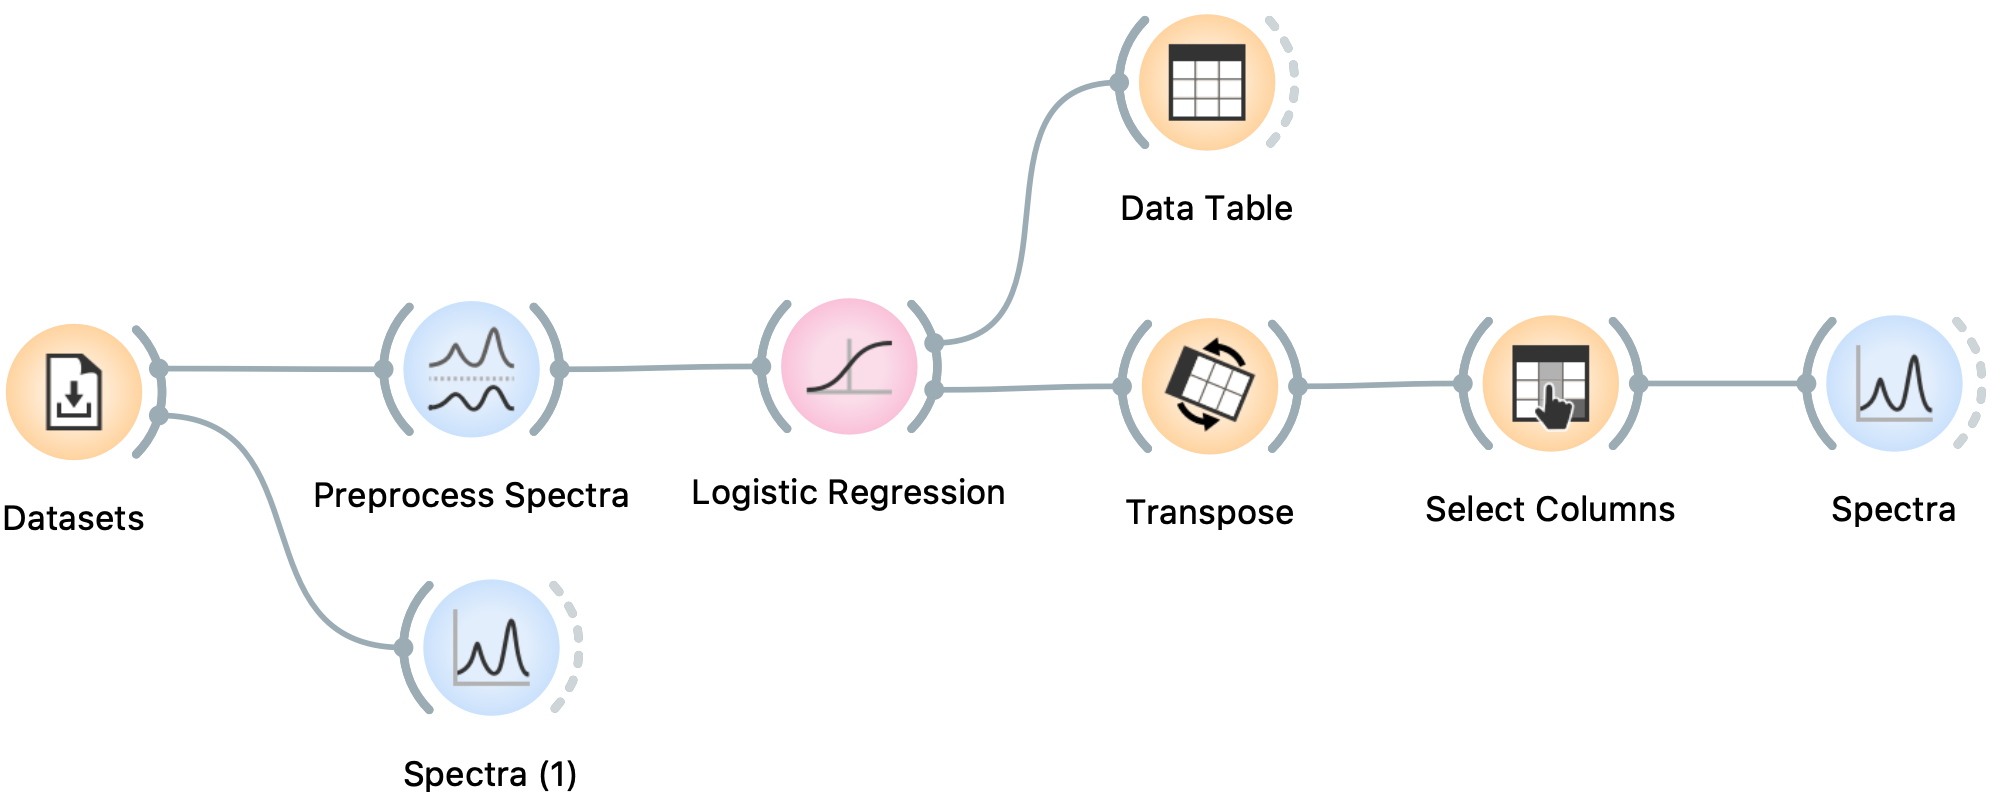
\includegraphics[width=1.1\textwidth]{graphics/ch-spectra_classification/sp_classification-fig3.png}%
  \label{fig:spectra_classification-fig3}
\end{wrapfigure}
But how does the model make its decisions? We already inspected a different model, classification tree, where each node represents a decision on a value of a column.  \widget{Logistic regression} works differently. On the training data it computes weights for all columns (wavelengths), which are then used for prediction, where values are multiplied with weights. To see the weights, connect \widget{Logistic Regression} to a \widget{Data Table}. 

\begin{wrapfigure}{o}{0.9\textwidth}
%  \centering
  \vspace{-0.5cm}
  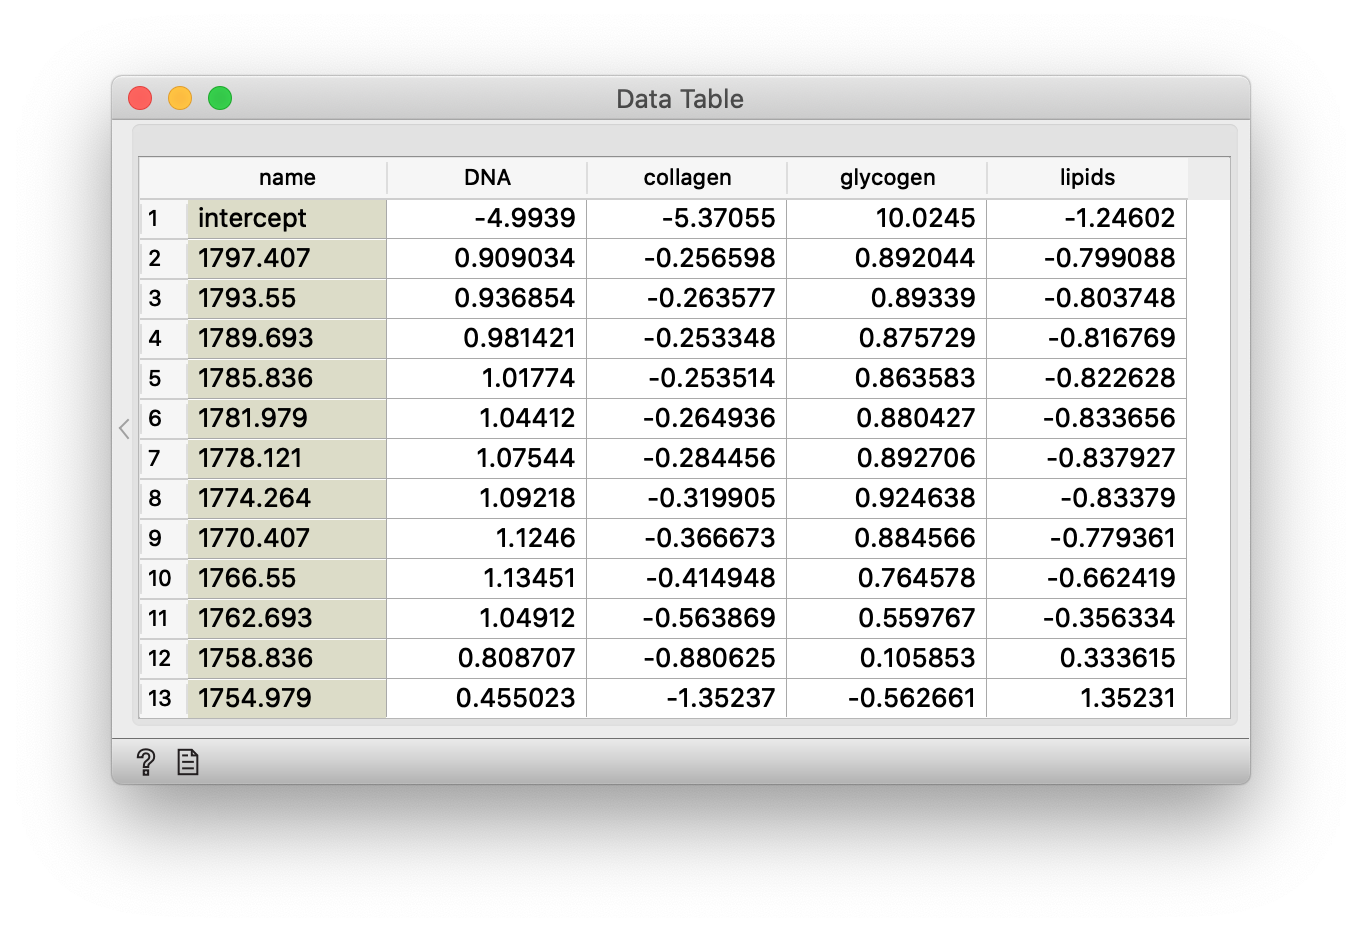
\includegraphics[width=0.9\textwidth]{graphics/ch-spectra_classification/sp_classification-fig4.png}
  \label{fig:spectra_classification-fig4}
\end{wrapfigure}
We get a table that is hard to understand. What if we visualize it? First, \widget{Transpose} the data. Then, use \widget{Select Columns} to make the visualization prettier: the widget removes the intercept. This changes the X axis.

Now, open \widget{Logistic Regression} and try changing parameters. What happens with the weights?

\vspace{2cm}

\huge
\noindent 2020.04.19 
THERE IS AN ERROR WHEN TRYING TO CREATE THIS WORKFLOW